\documentclass{fenicscourse}

% General math notation
\newcommand{\N}{\mathbb{N}}
\newcommand{\PP}{\mathbb{P}}
\newcommand{\QQ}{\mathbb{Q}}

% Math operators
\DeclareMathOperator{\ord}{ord}
\DeclareMathOperator{\Kern}{ker}
\DeclareMathOperator{\Image}{im}
\DeclareMathOperator{\spann}{span}
\DeclareMathOperator{\diam}{diam}


% Mesh and FEM notation
%\newcommand{\dx}{\, \mathrm{d} x}
%\newcommand{\ds}{\, \mathrm{d} s}
%\newcommand{\dS}{\, \mathrm{d} S}
\newcommand{\mesh}{\mathcal{T}}
\newcommand{\facets}{\mathcal{F}}
\newcommand{\inmesh}{\partial_i \mathcal{T}}
\newcommand{\exmesh}{\partial_e \mathcal{T}}

\newcommand{\jump}[1]{\llbracket #1 \rrbracket}
\newcommand{\avg}[1]{\langle #1 \rangle}
\newcommand{\meanvalue}[1]{\langle #1 \rangle}
\newcommand{\vect}[1]{\mathbf{#1}}

\newcommand{\gradhterm}[2]{(\nabla_h #1, \nabla_h #2)_{\Omega}}
\newcommand{\consterm}[2]{(\avg{\nabla_h #1} \dotn,\jump{#2})_{\inmesh}}
\newcommand{\penterm}[2]{( h^{-1} \jump{#1}, \jump{#2})_{\inmesh}}

\newcommand{\Ctr}{C_{\text{tr}}}

% Abbreviations for names etc
\newcommand{\apriori}{\emph{a~priori}}
\newcommand{\aposteriori}{\emph{a~posteriori}}

% Dimensions
\newcommand{\codesize}{\footnotesize}

% Environments
\DefineVerbatimEnvironment{code}{Verbatim}{frame=single,rulecolor=\color{blue}}

% Notes
\newcommand{\amnote}[1]{\todo[inline,color=blue!40]{\underline{AM:} #1}}
\newcommand{\mglnote}[1]{\todo[inline,color=red!40]{\underline{MGL:} #1}}
\newcommand{\alnote}[1]{\todo[inline,color=green!40]{\underline{AL:} #1}}
\newcommand{\mernote}[1]{\todo[inline,color=pink!40]{\underline{MER:} #1}}

% Special notation PI
\newcommand{\OmegaD}{\Omega_{0,\mathrm{D}}}
\newcommand{\OmegaN}{\Omega_{0,\mathrm{N}}}
\newcommand{\OmegaO}{\Omega_{_\mathrm{O}}}
\newcommand{\bfsigma}{{\pmb\sigma}}
\newcommand{\bfepsilon}{{\pmb\epsilon}}

% Special notation for PII
\newcommand{\bfu}{\boldsymbol{u}}
\newcommand{\bff}{\boldsymbol{f}}
\newcommand{\bfg}{\boldsymbol{g}}
\newcommand{\bfv}{\boldsymbol{v}}
\newcommand{\bfe}{\boldsymbol{e}}
\newcommand{\bfn}{\boldsymbol{n}}
\newcommand{\bfx}{\boldsymbol{x}}
\newcommand{\Oast}{\Omega^{\ast}}
\newcommand{\Vast}{\mathcal{V}^{\ast}}

%\newcommand{\meshast}{\mathcal{T}_{\ast}}
\newcommand{\pO}{\partial \Omega}
\newcommand{\meshast}{\mathcal{T}^{\ast}}
\newcommand{\Fast}{\mathcal{F}^{\ast}_{\Gamma}}
\newcommand{\piast}{\pi^{\ast}_h}
\newcommand{\tnast}{\tn_{\ast}}
\newcommand{\tnsip}{\tn_{\text{sip}}}
\newcommand{\tnsipast}{\tn_{\text{sip},\ast}}
\newcommand{\asip}{a^{\text{sip}}_h}

\newcommand{\mcF}{\mathcal{F}}
\newcommand{\mcT}{\mathcal{T}}
\newcommand{\mcV}{\mathcal{V}}
\newcommand{\mcE}{\mathcal{E}}
\newcommand{\mcN}{\mathcal{N}}
\newcommand{\mcC}{\mathcal{C}}
\newcommand{\mcA}{\mathcal{A}}
\newcommand{\tn}{|\mspace{-1mu}|\mspace{-1mu}|}
\newcommand{\Pzero}{P_h^{0,\mathrm{dc}}}
\newcommand{\Pone}{P_h^1}
\newcommand{\ndot}{\bfn \cdot}
\newcommand{\dotn}{\cdot \bfn}
\newcommand{\bfw}{\boldsymbol{w}}
\newcommand{\Wspace}{{\mathcal{V}_h}}

% Special notation for PIII
\newcommand{\nablan}{\partial_{\bfn}}
\newcommand{\OmcupOm}{\Omega_1 \cup \Omega_2}
\newcommand{\mcupm}{{\mathcal{T}^{\ast}_1} \cup \mesh_2}
%\newcommand{\mcupm}{{\meshast}_1 \cup \mesh_2}
%\newcommand{\meanvalue}[1]{\langle #1 \rangle_{\alpha}}
\newcommand{\ifnormalpha}[1]{\ifnorm{#1}{\alpha}}
\newcommand{\ifnorm}[2]{\| #1 \|_{#2,h,\Gamma}}
\newcommand{\tildev}{\widetilde{\bfv}}
\newcommand{\bfphi}{\boldsymbol{\phi}}
\newcommand{\picorr}{\pi^c}

% Math macros
\newcommand{\renni}[2]{\langle #2 ,\; #1 \rangle}


\begin{document}

\fenicslecture{Lecture 10: Discontinuous Galerkin methods
              for elliptic equations}
              {Andr\'e Massing \\ Marie E. Rognes}

%\linespread{1.5}

\begin{frame}
  \frametitle{The discontinuous Galerkin (DG) method uses
  discontinuous basis functions}
  \begin{columns}
    \begin{column}{0.3\textwidth}
      \only<1>{
      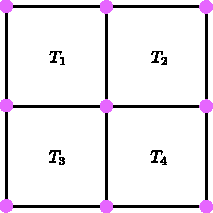
\includegraphics[width=1.0\textwidth]{pdf/box-mesh-before-split.pdf}
    }
    \only<2->{
      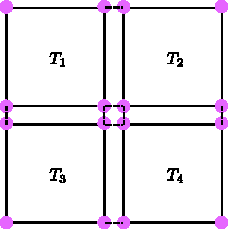
\includegraphics[width=1.0\textwidth]{pdf/box-mesh-after-split.pdf}
    }
    \end{column}
    \begin{column}{0.7\textwidth}
      \only<1-2>{
    \def\svgwidth{1.0\textwidth}
    \import{pdf/}{lin.pdf_tex}
  }
      \only<3->{
    \def\svgwidth{1.0\textwidth}
    \import{pdf/}{lin-dg.pdf_tex}
  }
    \end{column}
  \end{columns}
  \hspace{2em}
  \begin{equation*}
    V_h = P^k(\mcT_h) = \{ v_h \in L^2(\Omega): v_h|_{T} \in P^k(T)\; \foralls T \in
    \mcT_h\} 
  \end{equation*}
\end{frame}

\begin{frame}
  \frametitle{Discontinuous Galerkin: notation}

  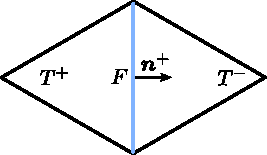
\includegraphics[scale=1.0]{pdf/dg-terms-interface.pdf}

  \begin{columns}[t]
    \begin{column}{0.5\textwidth}
      \alert{Average of a scalar field}: \\ $\avg{v} = \tfrac{1}{2} (v^+ + v^-)$ \\
      \bigskip

      \alert{Jump of a scalar field}: \\ $\jump{v} = (v^+ - v^-) n$
    \end{column}
    \begin{column}{0.5\textwidth}
      \alert{Average of a vector field}: \\ $\avg{B} = \tfrac{1}{2} (B^+ + B^-)$ \\
      \bigskip
      \alert{Jump of a vector field}: \\ $\jump{B} = (B^+ - B^-) \cdot n$
    \end{column}
  \end{columns}

  \bigskip

  {\alert{Jump identity} (Exercise for the reader!)}
  \begin{equation*}
    \jump{B v } = \jump{B} \avg{v}
    + \avg{B} \jump{v}
  \end{equation*}
\end{frame}

\begin{frame}
  \frametitle{The DG method eases mesh (h-) adaptivity}
  \begin{columns}[t]
    \begin{column}{0.3\textwidth}
    \only<1>{
      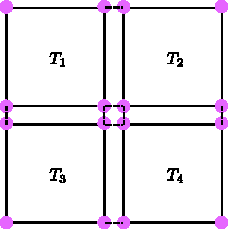
\includegraphics[width=1.0\textwidth]{pdf/box-mesh-after-split.pdf}
    }
    \only<2->{
      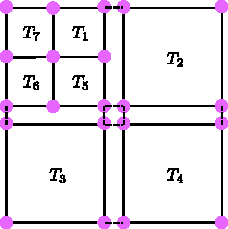
\includegraphics[width=1.0\textwidth]{pdf/box-mesh-after-split-h-refined.pdf}
    }
    \end{column}
    \begin{column}{0.7\textwidth}
      \only<1-2>{
    \def\svgwidth{1.0\textwidth}
    \import{pdf/}{lin-dg.pdf_tex}
  }
      \only<3->{
    \def\svgwidth{1.0\textwidth}
    \import{pdf/}{lin-dg-h-adapted.pdf_tex}
  }
    \end{column}
  \end{columns}
\end{frame}

\begin{frame}
  \frametitle{The DG method eases space (p-) adaptivity}
  \begin{columns}[t]
    \begin{column}{0.3\textwidth}
    \only<1>{
      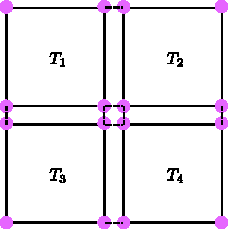
\includegraphics[width=1.0\textwidth]{pdf/box-mesh-after-split.pdf}
    }
    \only<2->{
      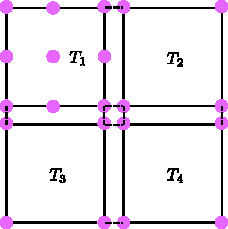
\includegraphics[width=1.0\textwidth]{pdf/box-mesh-after-split-p-refined.pdf}
    }
    \end{column}
    \begin{column}{0.7\textwidth}
      \only<1-2>{
    \def\svgwidth{1.0\textwidth}
    \import{pdf/}{lin-dg.pdf_tex}
  }
      \only<3->{
    \def\svgwidth{1.0\textwidth}
    \def\svgwidth{1.0\textwidth}
    \import{pdf/}{lin-dg-p-adapted.pdf_tex}
  }
    \end{column}
  \end{columns}
\end{frame}
%\begin{frame}
%  \frametitle{DG motivation}
%      \only<1>{
%    \def\svgwidth{1.0\textwidth}
%    \import{figures/trial-lecture/}{lin-dg.pdf_tex}
%  }
%      \only<2->{
%    \def\svgwidth{1.0\textwidth}
%    \def\svgwidth{1.0\textwidth}
%    \import{figures/trial-lecture/}{lin-dg-p-adapted.pdf_tex}
%  }
%\end{frame}


\begin{frame}
\frametitle{Poisson's equation revisited}

  Consider Poisson's equation again, now with homogeneous Dirichlet
  boundary conditions for simplicity
  \begin{equation*}
    \begin{split}
      - \Delta u &= f \,\,\, \quad \mbox{in } \Omega
      \\
      u &= 0 \quad \mbox{on } \partial \Omega
    \end{split}
  \end{equation*}

  \bigskip

  Assume that we have a mesh $\mesh = \{ T \}$ of $\Omega$

  \bigskip

  Let's also say that we would like the \alert{solution} $u$ and its
  \alert{flux} $\Grad u \cdot n$, where $n$ is the facet normal, to be
  \alert{continuous} across all facets of the mesh.

  \bigskip

  We are going to derive a discontinuous Galerkin (DG) formulation for
  this equations.

\end{frame}

\begin{frame}
  \frametitle{Deriving a DG formulation (i)}

  Multiply by a function $v$ and integrate over $\Omega$.
  \begin{equation*}
    \int_{\Omega} - \Delta u v \dx = \int_{\Omega} f v \dx
  \end{equation*}
  Integrate by parts? No, wait for it!

  \bigskip

  Assume that you have a mesh $\mesh$ of $\Omega$ with cells $\{T\}$
  and split left integral into sum over cell integrals:
  \begin{equation*}
    \sum_{T \in \mesh } \int_{T} - \Delta u v \dx = \int_{\Omega} f v \dx
  \end{equation*}
  Now integrate by parts!
  \begin{equation*}
    \sum_{T \in \mesh } \int_{T} \Grad u \cdot \Grad v \dx
    - \sum_{T \in \mesh } \int_{\partial T} \Grad u \cdot n \, v \ds
    = \int_{\Omega} f v \dx
  \end{equation*}
\end{frame}

\begin{frame}
  \frametitle{Deriving a DG formulation (ii)}

  \bigskip

  Each interior facet $e$ is shared by two cells ($T^+$ and $T^-$). We
  denote the set of all interior facets by $\facets_i$ and the set of
  all exterior (boundary) facets by $\facets_e$

  \bigskip

  Redistribute integrals over cell boundaries into integrals over
  facets $\facets$ as follows:
  \small
  \begin{equation*}
    \begin{split}
     \sum_{T \in \mesh } \int_{\partial T} \Grad u \cdot n \, v \ds
    =
    & \sum_{e \in \facets_i } \int_{e} (\Grad u^+ \cdot n^+ \, v^+  +  \Grad u^- \cdot n^- \, v^-) \ds  \\
    & + \sum_{e \in \facets_e } \int_{e} \Grad u \cdot n \, v \ds
    \end{split}
  \end{equation*}

  \normalsize
  Let us say that $n^+ = n$ (then $n^- = -n$), and rewrite
  \small
  \begin{equation*}
    \begin{split}
     \sum_{T \in \mesh } \int_{\partial T} \Grad u \cdot n \, v \ds
    =
    & \sum_{e \in \facets_i } \int_{e} (\Grad u^+ \cdot n \, v^+ - \Grad u^- \cdot n \, v^-) \ds  \\
    & + \sum_{e \in \facets_e } \int_{e} \Grad u \cdot n \, v \ds
    \end{split}
  \end{equation*}

  \normalsize
\end{frame}

\begin{frame}
  \frametitle{Discontinuous Galerkin: notation}

  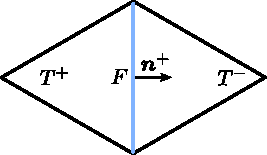
\includegraphics[scale=1.0]{pdf/dg-terms-interface.pdf}

  \begin{columns}[t]
    \begin{column}{0.5\textwidth}
      \alert{Average of a scalar field}: \\ $\avg{v} = \tfrac{1}{2} (v^+ + v^-)$ \\
      \bigskip

      \alert{Jump of a scalar field}: \\ $\jump{v} = (v^+ - v^-) n$
    \end{column}
    \begin{column}{0.5\textwidth}
      \alert{Average of a vector field}: \\ $\avg{B} = \tfrac{1}{2} (B^+ + B^-)$ \\
      \bigskip
      \alert{Jump of a vector field}: \\ $\jump{B} = (B^+ - B^-) \cdot n$
    \end{column}
  \end{columns}

  \bigskip

  {\alert{Jump identity} (Exercise for the reader!)}
  \begin{equation*}
    \jump{B v } = \jump{B} \avg{v}
    + \avg{B} \jump{v}
  \end{equation*}
\end{frame}


\begin{frame}
  \frametitle{Deriving a DG formulation (iii)}

  Now, let's introduce our shorthand notation for the jump:
  \begin{equation*}
    \begin{split}
     \sum_{T \in \mesh } \int_{\partial T} \Grad u \cdot n \, v \ds
    =
    \sum_{e \in \facets_i } \int_{e} \jump{\Grad u v} \ds
    + \sum_{e \in \facets_e } \int_{e} \Grad u \cdot n \, v \ds
    \end{split}
  \end{equation*}

  Use the jump identity to expand the first term
  \begin{equation*}
    \begin{split}
     \sum_{T \in \mesh } \int_{\partial T} \Grad u \cdot n \, v \ds
    =
    &\sum_{e \in \facets_i } \int_{e} \jump{\Grad u} \avg{v}
    + \avg{\Grad u} \jump{v} \ds \\
    &+ \sum_{e \in \facets_e } \int_{e} \Grad u \cdot n \, v \ds
    \end{split}
  \end{equation*}

\end{frame}

\begin{frame}
  \frametitle{Deriving a DG formulation (iv)}

  We want to weakly enforce
  \begin{itemize}
    \item
      Continuity of the flux: $\jump{\Grad u} = 0$ over all facets \\
      (Solution: Let the corresponding term vanish)
    \item
      Continuity of the solution $\jump{u} = 0$ over all facets \\
      (Solution: Add a corresponding term)
    \item
      Stability \\
      (Solution: add:
      \begin{equation*}
        S(u, v) = \sum_{e \in \facets} \int_{e} \tfrac{\beta}{h} \jump{u} \cdot \jump {v} \ds \quad
      \end{equation*}
      for some stabilization parameter $\beta > 0$ and mesh size $h$.)
  \end{itemize}
\end{frame}

\begin{frame}
  \frametitle{A symmetric interior penalty (SIP/DG) formulation for Poisson's equation}

  Find $u \in V_h = DG_k(\mesh)$ such that
  \begin{equation*}
    \begin{split}
      &\sum_{T \in \mesh } \int_{T} \Grad u \cdot \Grad v \dx \\
      &+ \sum_{e \in \facets_i } \int_{e} - \avg{\Grad u} \jump{v}  - \avg{\Grad v} \jump{u} + \tfrac{\alpha}{h} \jump{u} \cdot \jump {v} \ds \\
      & + \sum_{e \in \facets_e } \int_{e} - \Grad u \cdot n \, v - \Grad v \cdot n \, u + \tfrac{\alpha}{h} u \, v \ds
      = \int_{\Omega} f v \dx
    \end{split}
  \end{equation*}
  for all $v \in DG_k(\mesh)$.

\end{frame}

%\begin{frame}[t]
  \frametitle{The symmetric interior penalty method (SIP)}
  \begin{center}
    \begin{align*}
      a_h(u_h,v_h)
      &= 
      \sum_{T\in \mesh} \int_{T} \nabla u_h \cdot \nabla v_h \dx
      -\underbrace{
        \sum_{F \in \mcF} \int_{F}\avg{\nabla u_h}\dotn \jump{v_h}  \dS
      }_{\text{Consistency}}
      \\
        &\phantom{=}
      \uncover<2->{
        - \underbrace{
          \sum_{F \in \mcF} \int_{F}\avg{\nabla v_h}\dotn \jump{u_h} \dS
        }_{\text{Symmetry}}
      }
      \uncover<3->{
        + \underbrace{
          \sum_{F \in \mcF} \frac{\gamma}{h_F} \int_{F}\jump{u_h}
          \jump{v_h}  \dS
        }_{\text{Penalty}}
      }
      \\
      \only<4->{
      l_h(v_h)  & = 
        \uncover<4->{\int_{\Omega} fv_h \dx }
        \uncover<5->{
          - \sum_{F \in \mcF^b} \int_{F}\avg{\nabla v_h}\dotn g \dS
          + \sum_{F \in \mcF^b} \frac{\gamma}{h_F} \int_{F} g v_h  \dS
        }
      }
    \end{align*}
  \end{center}
\end{frame}

%\begin{frame}
  \frametitle{Split of SIP form into interior and boundary
  contribution}
  \vspace{-2em}
  \begin{center}
    \begin{align*}
      a_h(u_h,v_h)
      &=
      \sum_{T\in \mesh} \int_{T} \nabla u_h \cdot \nabla v_h \dx
      -\underbrace{
        \sum_{F \in \mcF^i} \int_{F}\avg{\nabla u_h}\dotn \jump{v_h}  \dS
      }_{\text{Consistency}}
      \\
        &\phantom{=}
        - \underbrace{
          \sum_{F \in \mcF^i} \int_{F}\avg{\nabla v_h}\dotn \jump{u_h} \dS
        }_{\text{Symmetry}}
        + \underbrace{
          \sum_{F \in \mcF^i} \frac{\gamma}{h_F} \int_{F}\jump{u_h}
          \jump{v_h}  \dS
        }_{\text{Penalty}}
      \\
        &\phantom{=}
      -\underbrace{
        \sum_{F \in \mcF^b} \int_{F}{\nabla u_h}\dotn {v_h}  \ds
      }_{\text{Consistency}}
        - \underbrace{
          \sum_{F \in \mcF^b} \int_{F}{\nabla v_h}\dotn {u_h} \ds
        }_{\text{Symmetry}}
      \\
        &\phantom{=}
        + \underbrace{
          \sum_{F \in \mcF^b} \frac{\gamma}{h_F} \int_{F}{u_h}
          {v_h}  \ds
        }_{\text{Penalty}}
    \end{align*}
  \end{center}
\end{frame}

\begin{frame}[fragile]
  \frametitle{Useful FEniCS tools for DG (I)}
  Access facet normals and local mesh size:
  \vspace{-1em}
  \begin{python}
mesh = UnitSquareMesh(8, 8)
n = FacetNormal(mesh)
h = mesh.hmin()
  \end{python}
  \bigskip
  Restrictions:
  \vspace{-1em}
  \begin{python}
V = FunctionSpace(mesh, "DG", 0)
f = Function(V)
f('+')
grad(f)('+')
  \end{python}
\end{frame}

\begin{frame}[fragile]
  \frametitle{Useful FEniCS tools for DG (II)}

  Average and jump:
  \vspace{-1em}
  \begin{python}
# Define it yourself
h_avg = (h('+') + h('-'))/2

# Or use built-in expression(s)
avg(h)

# This is v^+ - v^-
jump(v)

# This is (v^+ - v^-) n
jump(v, n)
  \end{python}

\end{frame}

\begin{frame}[fragile]
  \frametitle{Useful FEniCS tools for DG (III)}

Integration over sum of all \emph{interior} facets: \emp{dS}:
  \vspace{-1em}
\begin{python}
alpha = Constant(0.1)
u = TrialFunction(V)
v = TestFunction(V)
S = alpha/h_avg*dot(jump(v, n), jump(u, n))*dS
\end{python}
Integration over sum of all \emph{exterior} facets: \emp{ds}:
  \vspace{-1em}
\begin{python}
s = alpha/h*u*v*ds
\end{python}

\end{frame}

\begin{frame}
  \frametitle{FEniCS programming exercise}

  We consider our favorite Poisson problem on $\Omega = [0,1] \times
  [0,1]$ with $f = 1.0$.

  \bigskip

  Solve this PDE numerically by using the SIP/DG method. Try using
  different values for the stabilization parameter. How does the
  parameter affect the result?

  \bigskip

  Compare the solution with the solution obtained using the method of
  Lecture 02.
\end{frame}


\end{document}
